%--------------------------------------------------------------------
\medskip
\subsection{¿Qué arquitectura de referencia usaría? Justifique la respuesta}
Debido a que el sistema va dirigido a un departamento concreto de la compañía Mistery Shopping (al departamento antifraude) y haciendo uso de la Figura \ref{03-image} en la que se muestran las diferencias entre el Data Warehose de Inmon y de Kimball, la arquitectura de referencia que se va a usar para implementar el sistema es la basada en el Data Warehouse de Kimball. Se toma esta decisión por las características propias del enunciado: se trata de una solución para un departamento concreto; el coste inicial es muy bajo y, debido a que este es un caso práctico de una asignatura, el tiempo de desarrollo no es muy elevado; y el equipo de desarrollo no tiene una especificación alta.
\begin{figure}[!th]
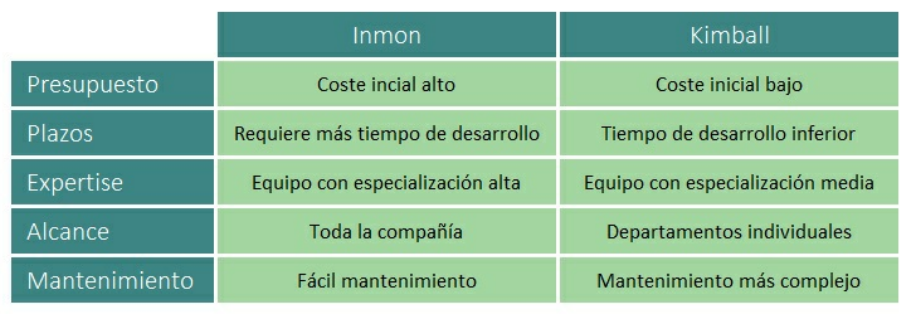
\includegraphics[scale=0.3]{03.png}
\centering
\caption{Diferencias entre el Data Warehouse de Inmon y de Kimball.}
\label{03-image}
\end{figure}
